\section{Dioden}
	Sperrstromdichte v. Si-Dioden: $10^{-11} \frac{A}{cm^2}$ \\
	\begin{tabular}{l l}
			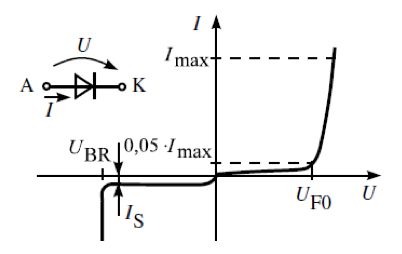
\includegraphics[width=8cm]{./images/Diode-Kennlinie.png}
		&	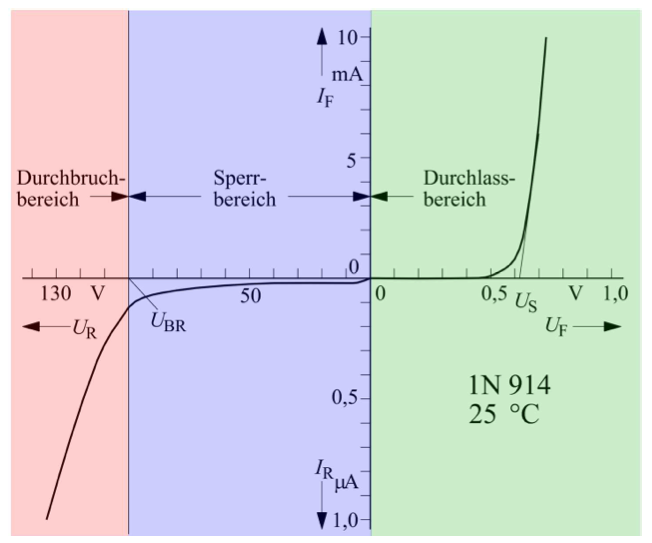
\includegraphics[width=8cm]{./images/Diode-Kennlinie-2.png}
	\end{tabular}
	
	\subsection{Kleinsignal-ESB}
		\begin{tabular}{l l}
			\multirow{5}{*}{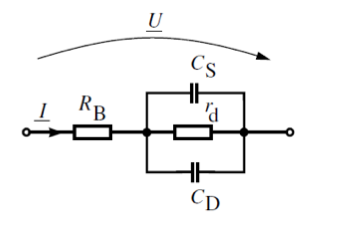
\includegraphics[width=4cm]{./images/Diode-KS-ESB.png}}
			& $R_B$: Bahnwiderstand (inkl. Zuleitung, Kontaktierung) \\
			& $r_d$: differentieller Widerstand des pn-Übergangs \\
			& $C_D$: Diffusionskapazität (bei pos. Diodenspannung) \\
			& $C_S$: Sperrschichtkapazität (bei neg. Diodenspannung)\\
			& $r_d=\frac{dU}{dI}$ (Tangentensteigung im AP) \\
		\end{tabular}
	
	\subsection{Grosssignal-ESB}
		\begin{tabular}{l l}
			\multirow{6}{*}{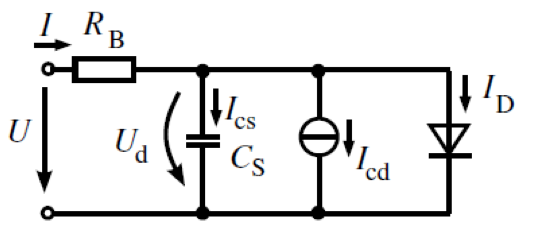
\includegraphics[width=4cm]{./images/Diode-GS-ESB.png}}
			& Gleichstromwiderstand $R_D = \frac{U_0}{I_0}$ (im AP)\\
			& $I=I_S \cdot (e^{\frac{U}{m \cdot U_T}}-1)$ \\
			& $I_S$: Sättigungssperrstrom (Bereich: $pA$)\\
			& $m$: Emissionskoeffizient (meistens: $m=1$) \\
			& $U_T=\frac{kT}{q} \approx 26mV$ \\
			& beim Umschalten bewirken die Kapazitäten $C_S$ und $C_D$ eine Verzögerung \\
		\end{tabular}
		
	\subsection{Temperaturverhalten}
		Faustregel: Durchflusspannung $U_{F0}$ ändert um $-2 \frac{mV}{K}$! \\
		$U_T$ in Abhängigkeit der Temperatur: 
		$U_T(T) = \frac{k \cdot T}{q} = 86,142 \frac{\mu \text{V}}{\text{K}} \cdot T$
		mit $U_T(300 \: K) = 26 mV$ \\
		Der Sperrstrom verdoppelt sich je Temperaturunterschied à $10K$
	
	
	\subsection{Spezielle Dioden und Anwendungen}
		\subsubsection{PIN-Diode}
			Für höhere Spannungsfestigkeit wird eigenleitende Halbleiterzone, die sog. 
			Intrinsic-Zone zwischen p- und n-dotierte Zone gelegt. Die Intrinsic-Zone
			ist im Sperrbetrieb sehr hochohmig und reduziert somit die el. Feldstärke
			auf ein akzeptables Mass.
		
		\subsubsection{Kapazitätsdiode}
			Kapazitätsdioden (Varicaps) werden in Sperrichtung betrieben. Die 
			Kapazität hängt dabei von der Spannung $U_{SP}$ ab.
			Anwendung: Einstellen der Schwingfrequenz in Oszillatoren \\
			
		\subsubsection{Tunneldiode}
			Tunneldioden besitzen eine sehr hohe Störstellenkonzentration und einen
			steilen Dotierungsverlauf. 
			
		\subsubsection{Zener-Diode}
		\begin{tabular}{l l}
			\multirow{5}{*}{
			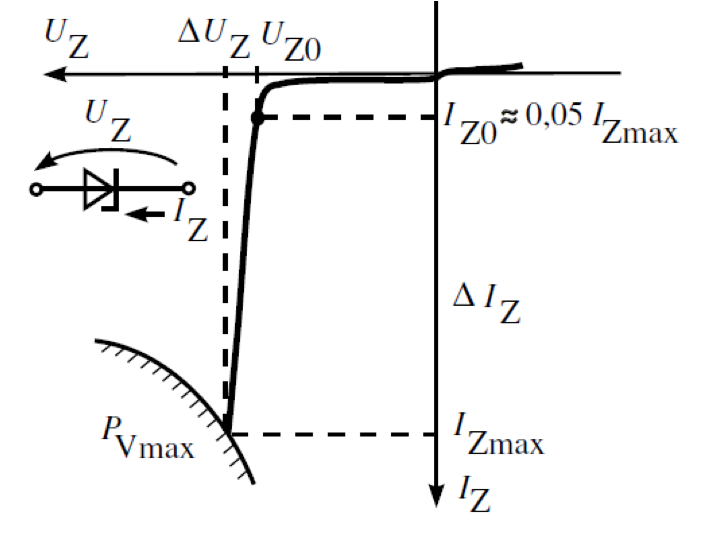
\includegraphics[width=6cm]{./images/zdiode-kennlinie.png}} & \\
			& Anstieg der Durchbruchkennlinie bei spezieller Dotierung \\
			& Anwendung: Spannungsbegrenzung und -stabilisierung \\ & \\ & \\
		\end{tabular} \\ 
		
		\subsubsection{Schottky-Diode}
			ToDo!